\documentclass[14pt]{extbook}
\usepackage{multicol, enumerate, enumitem, hyperref, color, soul, setspace, parskip, fancyhdr} %General Packages
\usepackage{amssymb, amsthm, amsmath, bbm, latexsym, units, mathtools} %Math Packages
\everymath{\displaystyle} %All math in Display Style
% Packages with additional options
\usepackage[headsep=0.5cm,headheight=12pt, left=1 in,right= 1 in,top= 1 in,bottom= 1 in]{geometry}
\usepackage[usenames,dvipsnames]{xcolor}
\usepackage{dashrule}  % Package to use the command below to create lines between items
\newcommand{\litem}[1]{\item#1\hspace*{-1cm}\rule{\textwidth}{0.4pt}}
\pagestyle{fancy}
\lhead{Progress Quiz 9}
\chead{}
\rhead{Version B}
\lfoot{8590-6105}
\cfoot{}
\rfoot{Fall 2020}
\begin{document}

\begin{enumerate}
\litem{
Solve the rational equation below. Then, choose the interval(s) that the solution(s) belongs to.\[ \frac{-3x}{4x -6} + \frac{-5x^{2}}{-8x^{2} +28 x -24} = \frac{-4}{-2x + 4} \]\begin{enumerate}[label=\Alph*.]
\item \( x \in [-9.18,-6.04] \)
\item \( x_1 \in [2.95, 4.01] \text{ and } x_2 \in [-10.29,-6.29] \)
\item \( x \in [1.1,2.44] \)
\item \( x_1 \in [2.95, 4.01] \text{ and } x_2 \in [-4.5,8.5] \)
\item \( \text{All solutions lead to invalid or complex values in the equation.} \)

\end{enumerate} }
\litem{
Determine the domain of the function below.\[ f(x) = \frac{5}{15x^{2} +27 x + 12} \]\begin{enumerate}[label=\Alph*.]
\item \( \text{All Real numbers except } x = a, \text{ where } a \in [-20.09, -19.99] \)
\item \( \text{All Real numbers except } x = a \text{ and } x = b, \text{ where } a \in [-1.04, -0.84] \text{ and } b \in [-0.81, -0.71] \)
\item \( \text{All Real numbers except } x = a, \text{ where } a \in [-1.04, -0.84] \)
\item \( \text{All Real numbers.} \)
\item \( \text{All Real numbers except } x = a \text{ and } x = b, \text{ where } a \in [-20.09, -19.99] \text{ and } b \in [-9.08, -8.92] \)

\end{enumerate} }
\litem{
Solve the rational equation below. Then, choose the interval(s) that the solution(s) belongs to.\[ \frac{-30}{25x + 20} + 1 = \frac{-30}{25x + 20} \]\begin{enumerate}[label=\Alph*.]
\item \( x_1 \in [-1.5, -0.6] \text{ and } x_2 \in [-3.8,0.2] \)
\item \( x \in [0.6,1.1] \)
\item \( \text{All solutions lead to invalid or complex values in the equation.} \)
\item \( x \in [-0.8,1.2] \)
\item \( x_1 \in [-1.5, -0.6] \text{ and } x_2 \in [0.8,2.8] \)

\end{enumerate} }
\litem{
Solve the rational equation below. Then, choose the interval(s) that the solution(s) belongs to.\[ \frac{-52}{-78x + 104} + 1 = \frac{-52}{-78x + 104} \]\begin{enumerate}[label=\Alph*.]
\item \( x \in [1.33,2.33] \)
\item \( x_1 \in [1, 2] \text{ and } x_2 \in [1.33,2.33] \)
\item \( x_1 \in [-1.7, -1] \text{ and } x_2 \in [1.33,2.33] \)
\item \( \text{All solutions lead to invalid or complex values in the equation.} \)
\item \( x \in [-1.7,-1] \)

\end{enumerate} }
\litem{
Choose the graph of the equation below.\[ f(x) = \frac{1}{(x + 1)^2} - 2 \]\begin{enumerate}[label=\Alph*.]
\begin{multicols}{2}\item 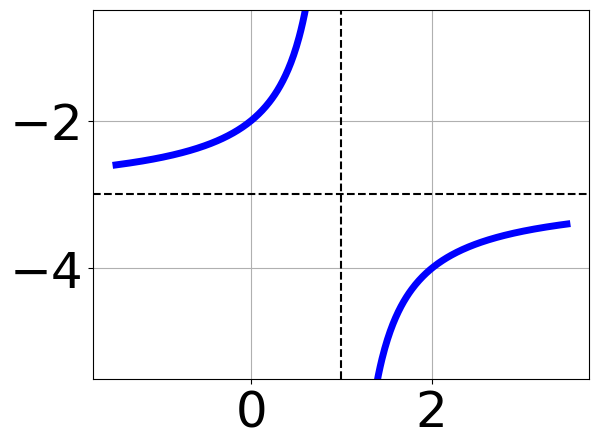
\includegraphics[width = 0.3\textwidth]{../Figures/rationalEquationToGraphCopyAB.png}\item 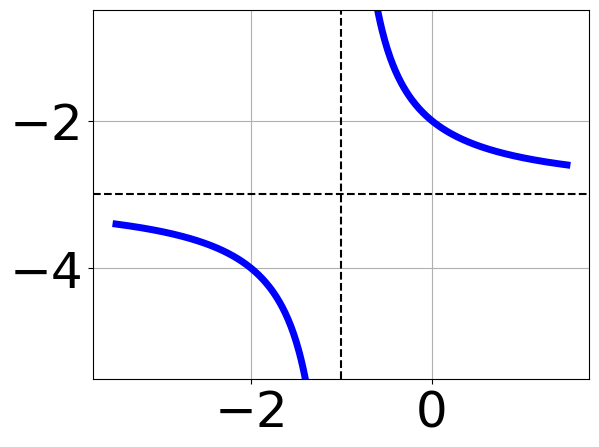
\includegraphics[width = 0.3\textwidth]{../Figures/rationalEquationToGraphCopyBB.png}\item 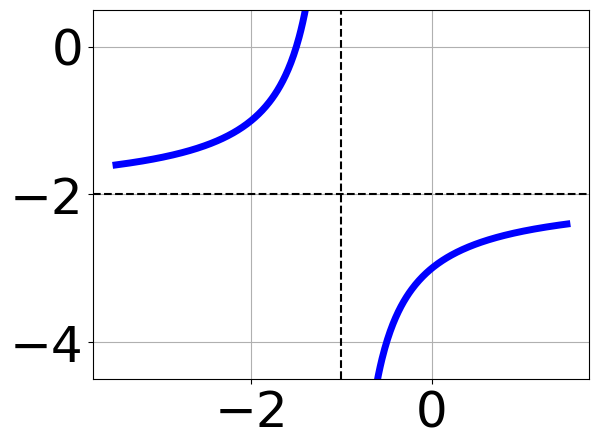
\includegraphics[width = 0.3\textwidth]{../Figures/rationalEquationToGraphCopyCB.png}\item 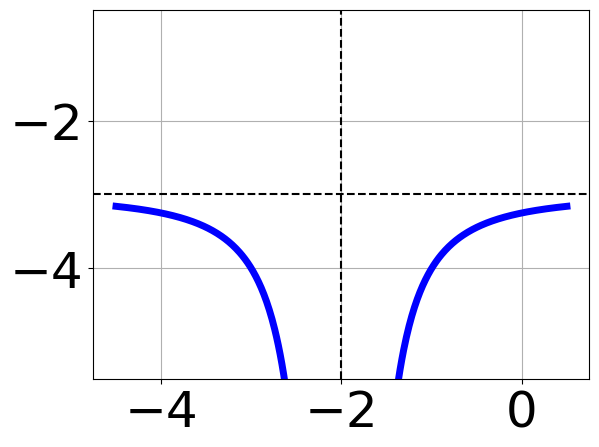
\includegraphics[width = 0.3\textwidth]{../Figures/rationalEquationToGraphCopyDB.png}\end{multicols}\item None of the above.
\end{enumerate} }
\litem{
Determine the domain of the function below.\[ f(x) = \frac{3}{18x^{2} +21 x -30} \]\begin{enumerate}[label=\Alph*.]
\item \( \text{All Real numbers except } x = a, \text{ where } a \in [-19, -16] \)
\item \( \text{All Real numbers except } x = a \text{ and } x = b, \text{ where } a \in [-19, -16] \text{ and } b \in [29, 33] \)
\item \( \text{All Real numbers.} \)
\item \( \text{All Real numbers except } x = a \text{ and } x = b, \text{ where } a \in [-2, 0] \text{ and } b \in [0.83, 2.83] \)
\item \( \text{All Real numbers except } x = a, \text{ where } a \in [-2, 0] \)

\end{enumerate} }
\litem{
Choose the equation of the function graphed below.
\begin{center}
    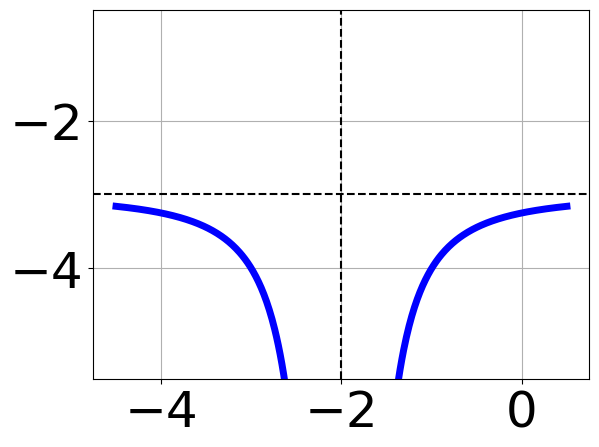
\includegraphics[width=0.5\textwidth]{../Figures/rationalGraphToEquationCopyB.png}
\end{center}
\begin{enumerate}[label=\Alph*.]
\item \( f(x) = \frac{-1}{(x + 2)^2} - 4 \)
\item \( f(x) = \frac{1}{(x - 2)^2} - 4 \)
\item \( f(x) = \frac{1}{x - 2} - 4 \)
\item \( f(x) = \frac{-1}{x + 2} - 4 \)
\item \( \text{None of the above} \)

\end{enumerate} }
\litem{
Choose the equation of the function graphed below.
\begin{center}
    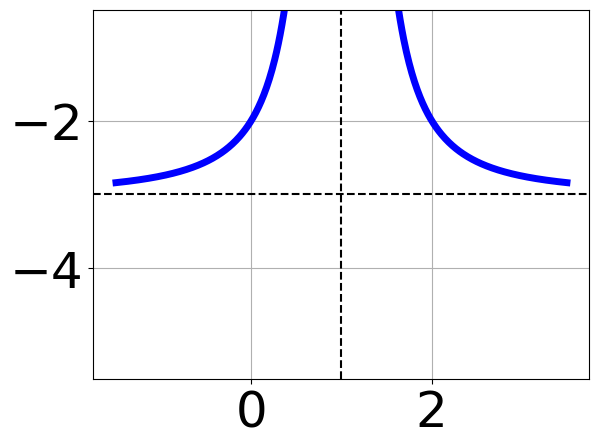
\includegraphics[width=0.5\textwidth]{../Figures/rationalGraphToEquationB.png}
\end{center}
\begin{enumerate}[label=\Alph*.]
\item \( f(x) = \frac{1}{x + 2} + 3 \)
\item \( f(x) = \frac{1}{(x + 2)^2} + 3 \)
\item \( f(x) = \frac{-1}{x - 2} + 3 \)
\item \( f(x) = \frac{-1}{(x - 2)^2} + 3 \)
\item \( \text{None of the above} \)

\end{enumerate} }
\litem{
Choose the graph of the equation below.\[ f(x) = \frac{1}{(x + 3)^2} + 1 \]\begin{enumerate}[label=\Alph*.]
\begin{multicols}{2}\item 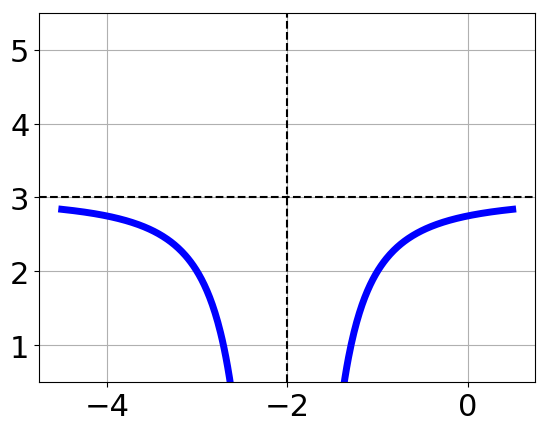
\includegraphics[width = 0.3\textwidth]{../Figures/rationalEquationToGraphAB.png}\item 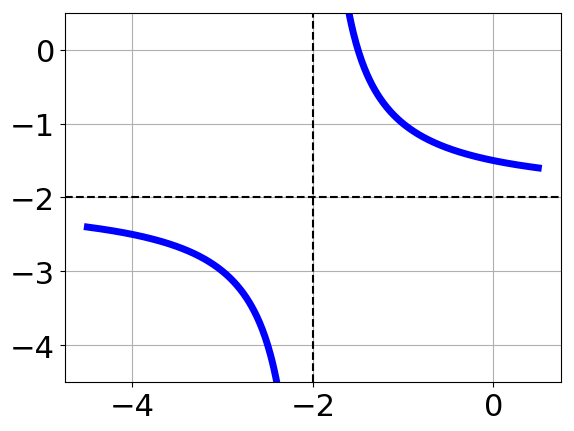
\includegraphics[width = 0.3\textwidth]{../Figures/rationalEquationToGraphBB.png}\item 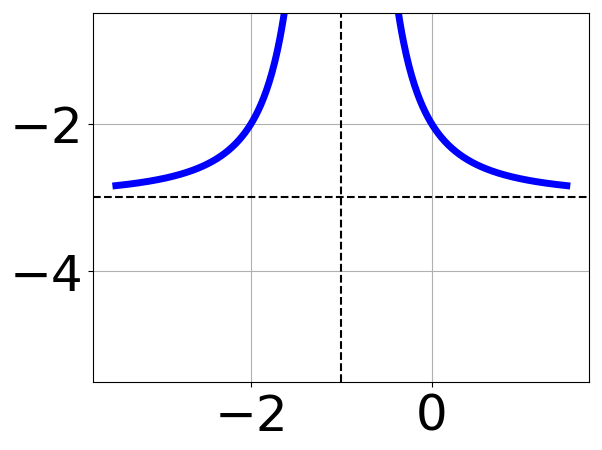
\includegraphics[width = 0.3\textwidth]{../Figures/rationalEquationToGraphCB.png}\item 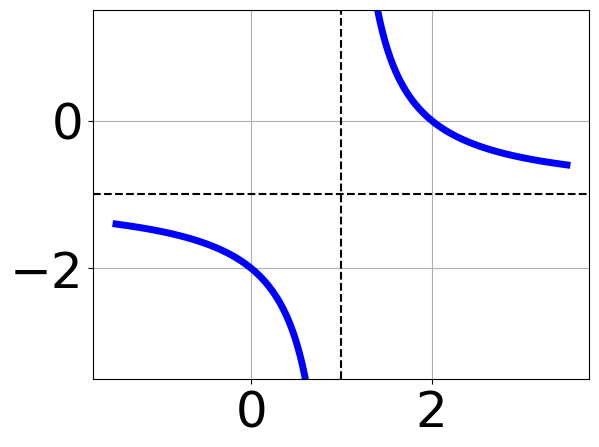
\includegraphics[width = 0.3\textwidth]{../Figures/rationalEquationToGraphDB.png}\end{multicols}\item None of the above.
\end{enumerate} }
\litem{
Solve the rational equation below. Then, choose the interval(s) that the solution(s) belongs to.\[ \frac{-3x}{-4x + 2} + \frac{-3x^{2}}{-12x^{2} +18 x -6} = \frac{-3}{3x -3} \]\begin{enumerate}[label=\Alph*.]
\item \( x_1 \in [0.22, 0.94] \text{ and } x_2 \in [-0.4,3.1] \)
\item \( \text{All solutions lead to invalid or complex values in the equation.} \)
\item \( x \in [0.67,1.51] \)
\item \( x \in [-1.32,-0.49] \)
\item \( x_1 \in [0.22, 0.94] \text{ and } x_2 \in [-3.8,-0.7] \)

\end{enumerate} }
\end{enumerate}

\end{document}